\documentclass[10pt,a4paper]{article}
\usepackage[utf8]{inputenc}
\usepackage[T1]{fontenc}
\usepackage{lmodern}
\usepackage[spanish]{babel}
\usepackage[margin=1.8cm]{geometry}
\usepackage{array,tabularx,booktabs}
\usepackage{graphicx}
\usepackage{float}
\usepackage[hidelinks]{hyperref}
\setlength{\parindent}{0pt}
\setlength{\parskip}{4pt}
\newcolumntype{Y}{>{\raggedright\arraybackslash}X}
\begin{document}
% Carátula: se incluye la primera página de caratula.tex a página completa.
% Se usa graphicx (clave page=) en lugar de pdfpages para no requerir paquetes extra.
% 2pt menos de alto: si la imagen mide exactamente \paperheight, no cabe por
% redondeo y LaTeX inserta una página en blanco antes de la carátula.
\newgeometry{margin=0pt,noheadfoot}
\thispagestyle{empty}%
\noindent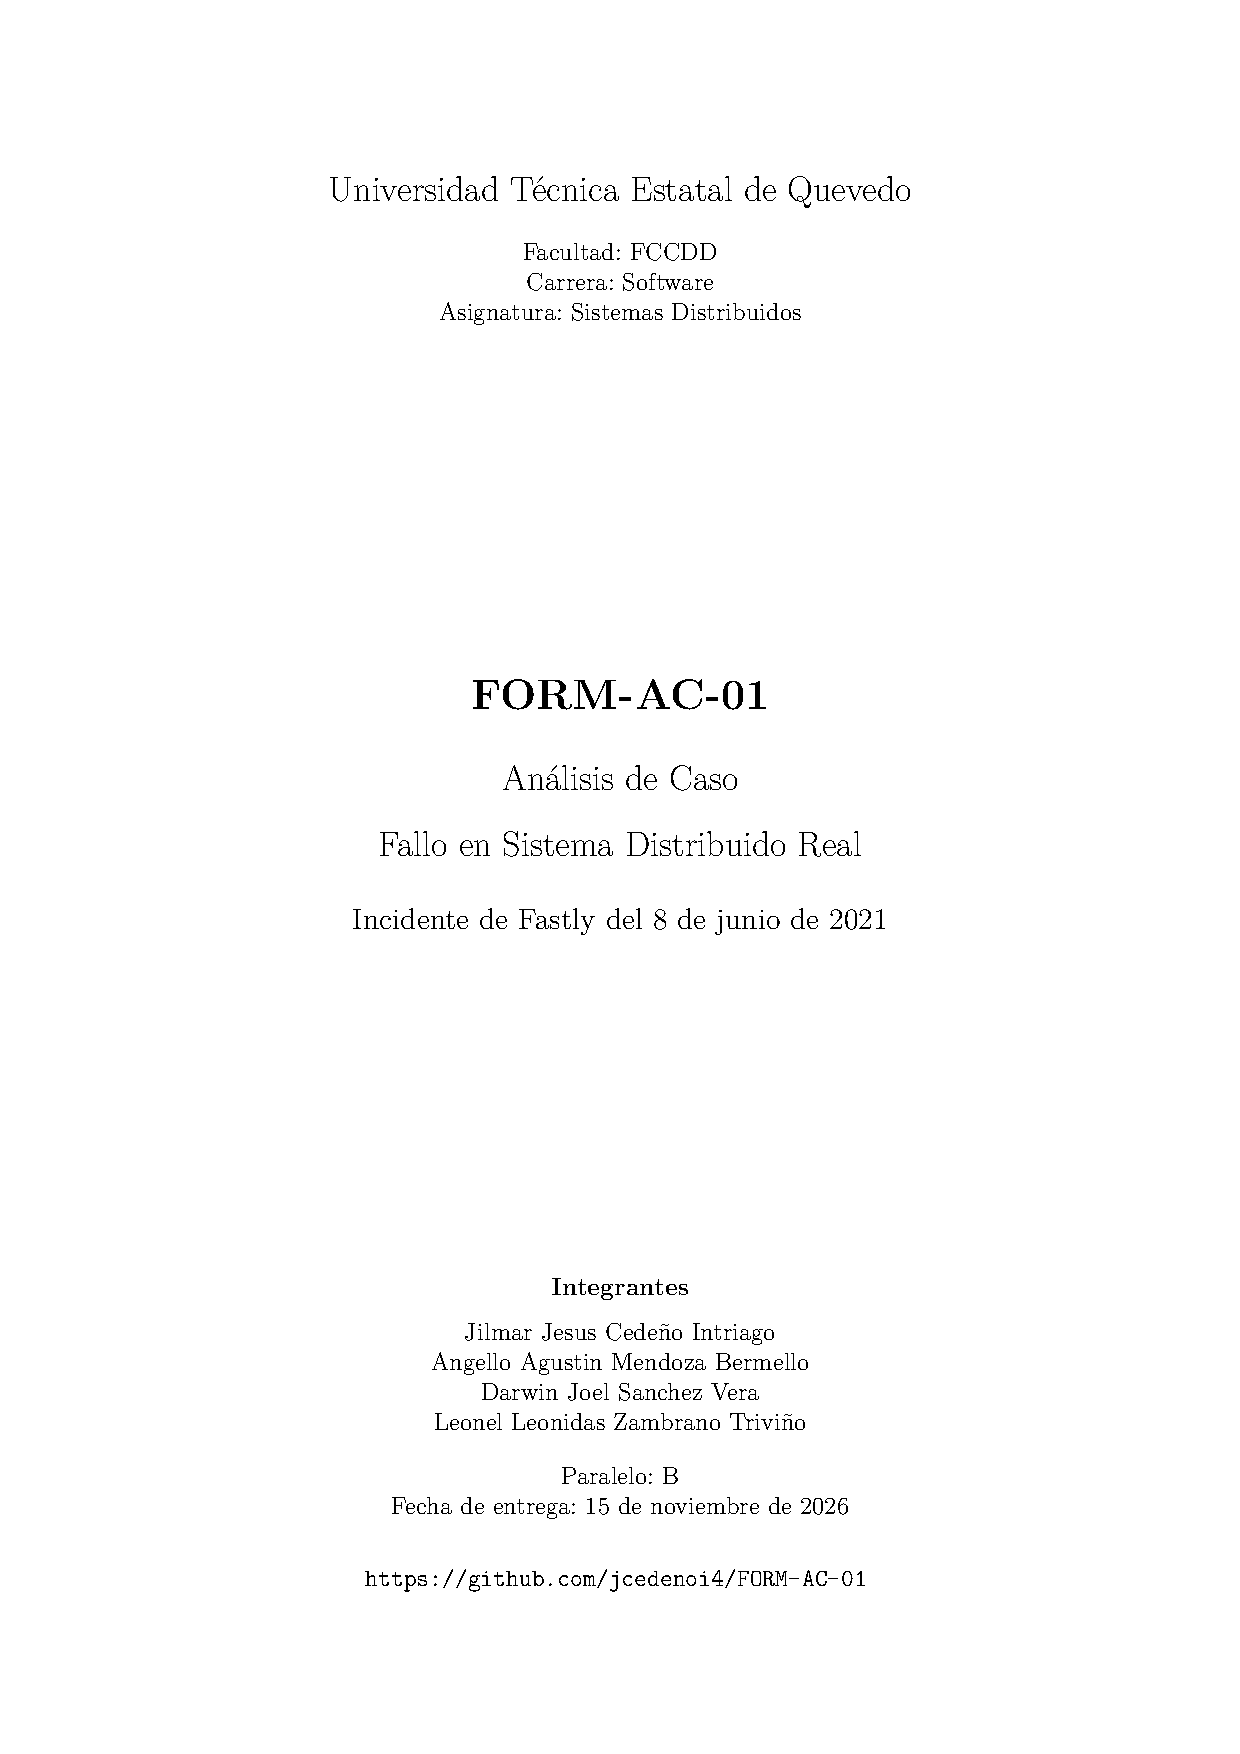
\includegraphics[page=1,width=\paperwidth,height=\dimexpr\paperheight-2pt\relax]{entrega/Entrega_SGA_FORM-AC-01.pdf}%
\clearpage
\restoregeometry
\setcounter{page}{1}
\section*{Descripción del incidente y línea de tiempo}
Fastly ofrece una red de distribución de contenido (CDN): sus servidores distribuidos entregan contenido de los sitios clientes. El 8 de junio de 2021, un cambio válido de configuración activó un defecto introducido en un despliegue iniciado el 12 de mayo. El 85\,\% de la red devolvió errores. El informe indica operación normal del 95\,\% de la red en 49 minutos; esto no equivale al cierre total del incidente~\cite{fastly2021}.

\begin{center}
\small
\begin{tabularx}{\linewidth}{@{}llY@{}}
\toprule
Hora & Zona & Acontecimiento del 8 de junio de 2021 \\
\midrule
09:47 & UTC & Inicio de la interrupción global. \\
09:48 & UTC & El monitoreo detecta el fallo. \\
09:58 & UTC & Publicación del aviso de estado. \\
10:27 & UTC & Ingeniería identifica la configuración desencadenante. \\
10:36 & UTC & Los servicios afectados comienzan a recuperarse. \\
11:00 & UTC & La mayoría de los servicios se ha recuperado. \\
12:35 & UTC & Incidente mitigado. \\
12:44 & UTC & Aviso de estado marcado como resuelto. \\
17:25 & UTC & Comienza el despliegue de la corrección permanente. \\
\bottomrule
\end{tabularx}
\end{center}
\textbf{Duración:} desde las 09:47 hasta la mitigación transcurren 2 h 48 min; hasta el cierre del aviso, 2 h 57 min. Son diferencias calculadas entre las horas oficiales, no una caída uniforme de toda la red. Fuente de la tabla: Fastly~\cite{fastly2021}. Ecuador continental: UTC$-$5.

\section*{Causas raíz y diagrama de Ishikawa}

El 8 de junio de 2021, un cliente cambió la configuración de su servicio y, sin querer, activó
un error que Fastly había instalado el 12 de mayo. El error estuvo 27 días dormido. Ese día el
85\,\% de la red dejó de responder bien y el servicio volvió a la normalidad en 49
minutos~\cite{fastly2021}. Cook explica que en estos sistemas ningún fallo tiene una sola
causa: el accidente ocurre cuando varios fallos pequeños se juntan~\cite[p.~2]{cook1998}. Por
eso aquí se separa el cambio que lo activó de las condiciones que lo empeoraron.

El error no era fácil de ver: pasó las pruebas que Fastly hizo antes de publicarlo y solo
apareció con la configuración real del cliente. Gunawi y sus coautores cuentan que eso es
común en las actualizaciones: se prueban en un ambiente controlado y fallan al entrar en el
sistema completo~\cite[p.~5]{gunawi2016}. Yuan y sus coautores calcularon que el 58\,\% de las
caídas más graves que estudiaron se habría detectado con pruebas sencillas del código que
maneja los errores~\cite[p.~250]{yuan2014}.

Lo que hizo grande el fallo fue la repetición. Xu y sus coautores muestran que un mismo error
de configuración se copia en miles de servidores y queda guardado, así que tener copias no
ayuda y reiniciar tampoco lo arregla~\cite[p.~619]{xu2016}. Gunawi y sus coautores agregan que,
si todos los servidores usan el mismo programa, un solo error los afecta a todos al mismo
tiempo~\cite[p.~6]{gunawi2016}.

El aviso llegó rápido, en un minuto, pero saber cuál era la configuración culpable tomó
cuarenta: el informe marca el inicio a las 09:47 y la identificación a las
10:27~\cite{fastly2021}. Gunawi y sus coautores advierten que el sistema que vigila también
puede fallar, porque el código que revisa los errores tiene errores~\cite[p.~8]{gunawi2016}.

La Figura~\ref{fig:causas} agrupa las causas en seis grupos y usa el color para separar tres
niveles: naranja para lo que activó el fallo, rojo para el error que estaba dormido y azul para
lo que lo empeoró. Los grupos no están aislados: Cook insiste en que hacen falta varios fallos
a la vez~\cite[p.~1]{cook1998} y Fastly reconoce que, aunque las condiciones eran raras, debió
preverlo~\cite{fastly2021}.

\emph{Nota de transparencia: esta sección se redactó con apoyo de un asistente de inteligencia
artificial. Las cifras y citas se contrastaron con las fuentes de la carpeta
\texttt{artículos científicos/} y el diagrama es de elaboración propia.}

% la figura y la tabla de riesgos van juntas en una pagina nueva
\clearpage
\begin{figure}[t]
  \centering
  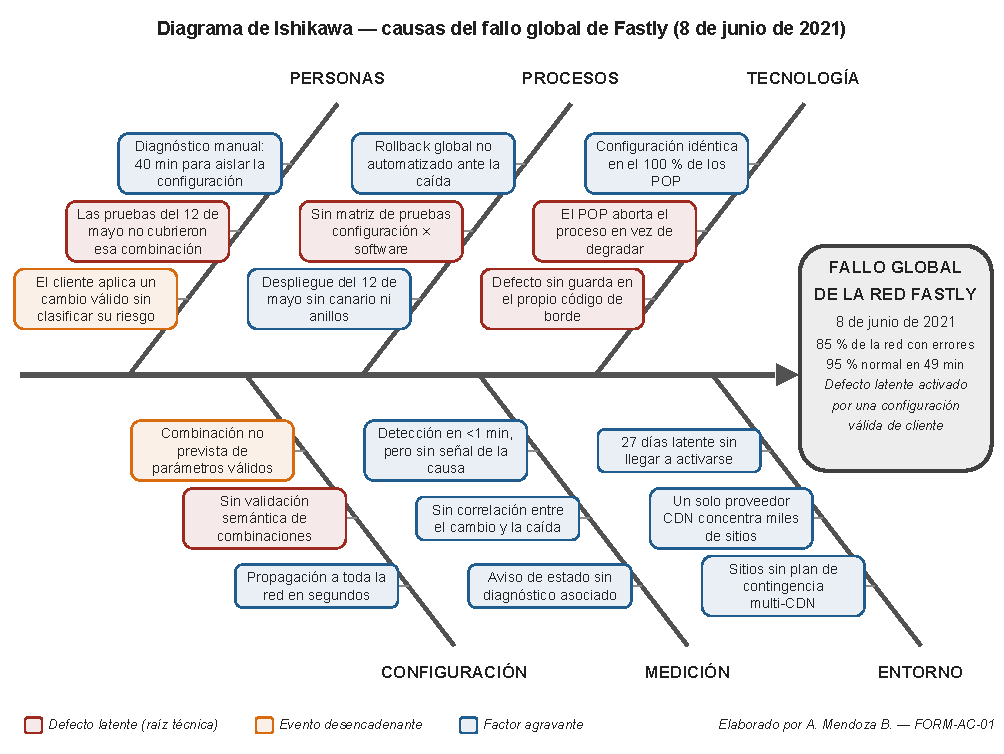
\includegraphics[width=\linewidth]{../diagramas/causas-fastly.pdf}
  \caption{Diagrama de Ishikawa del fallo del 8 de junio de 2021. Elaboración propia en
  draw.io; el archivo editable se conserva en \texttt{diagramas/causas-fastly.drawio}.}
  \label{fig:causas}
\end{figure}

\subsection*{Tres riesgos de SGIRI vinculados a estas causas}

\emph{SGIRI es el Sistema de Gestión de Incidencias que desarrollo como PFC: backend en Spring
Boot con PostgreSQL, frontend en Angular, tickets con estados y SLA, y adjuntos en Cloudinary.}

\begingroup
\small
\renewcommand{\arraystretch}{1.15}
\begin{tabularx}{\linewidth}{@{}YY@{}}
\toprule
Riesgo del PFC y consecuencia (categoría del diagrama) & Medida preventiva comprobable en TA-PFC-E1 \\
\midrule
\textbf{SGIRI:} un cambio válido en las reglas que mueven un ticket de un estado a otro (nuevo,
asignado, en proceso, resuelto, cerrado) puede dejarlo sin salida y con el reloj del SLA
corriendo (personas y procesos).
& Guardar cada versión de las reglas y probar todas las transiciones posibles antes de
activarlas; forzar una transición no permitida y comprobar que el ticket conserva su estado y
que el contador del SLA no salta. Validar la configuración al inicio es justamente lo que
falta en muchos sistemas~\cite[p.~619]{xu2016}. \\
\addlinespace
\textbf{SGIRI:} una versión nueva del backend con una credencial o una URL de base de datos mal
puesta no arranca y, al ser una sola instancia, el sistema entero queda caído (tecnología).
& Desplegar primero en un entorno de prueba, comprobar el arranque y la respuesta de salud
antes de pasar el tráfico, y conservar el paquete anterior para revertir. Tener copias no basta
si no se completa la cadena de detección, cambio y respaldo~\cite[p.~5]{gunawi2016}. \\
\addlinespace
\textbf{SGIRI:} los adjuntos dependen de Cloudinary; si el servicio externo falla o tarda, el
alta de la incidencia termina en error 500 y el ticket no se registra (entorno).
& Separar la subida del alta: guardar el ticket primero y subir el adjunto después, con tiempo
límite y reintento; comprobar con Cloudinary bloqueado que el ticket igual se registra. Lo
peor es abortar en vez de degradar~\cite[p.~250]{yuan2014}, y provocar el fallo a propósito es
la forma de verificarlo~\cite{basiri2016}. \\
\bottomrule
\end{tabularx}
\endgroup

% ============================================================
% Sección: Relación con la Unidad 1
% Responsable: Sánchez Vera Darwin Joel
% ============================================================
\section*{Relación con la Unidad 1}
\textbf{Transparencia de distribución.} La transparencia ante fallos busca que el usuario no note que una parte del sistema dejó de funcionar~\cite{vansteen2016}. En una CDN, si un servidor falla, otro debería atender la petición sin que el visitante lo perciba. El 8 de junio ocurrió lo contrario: el 85\,\% de la red devolvió errores~\cite{fastly2021} y los visitantes de sitios como Reddit recibieron errores HTTP 503 \textit{Service Unavailable}~\cite{medina2021thousandeyes}. Un proveedor intermedio que el usuario normalmente no ve quedó expuesto en su pantalla.

\textbf{Teorema CAP.} El teorema relaciona tres propiedades: consistencia (C, todos los nodos muestran los mismos datos), disponibilidad (A, toda petición recibe una respuesta válida) y tolerancia a particiones (P, el sistema sigue operando aunque se corte la comunicación entre nodos). Brewer aclara que elegir entre C y A solo es necesario cuando existe una partición~\cite{brewer2012}. En el incidente se perdió la disponibilidad: los servidores respondían, pero con errores~\cite{fastly2021,medina2021thousandeyes}. Sin embargo, no fue un sacrificio de diseño ante una partición: las fuentes no describen una división de la red, sino un defecto de software activado por una configuración válida~\cite{fastly2021}. Por eso el caso no encaja en el dilema clásico C frente a A; muestra que la disponibilidad también se pierde sin partición cuando todos los nodos comparten el mismo defecto.

\textbf{Tolerancia a fallos.} El mecanismo que no funcionó fue la redundancia por replicación: muchos servidores distribuidos que se respaldan entre sí para que el fallo de uno no afecte el servicio. Esta redundancia supone que los nodos fallan de forma independiente; Avižienis et al.\ explican que las copias idénticas no toleran defectos de desarrollo persistentes, que requieren diversidad de diseño~\cite{avizienis2004}. En Fastly, todos los nodos ejecutaban el software desplegado desde el 12 de mayo con el mismo defecto latente, y la configuración de un cliente lo activó a la vez en el 85\,\% de la red~\cite{fastly2021}: un fallo de modo común. La detección sí funcionó (09:48 UTC), pero identificar la configuración tomó 40 minutos (10:27 UTC)~\cite{fastly2021}. Esto se relaciona con dos causas: las pruebas no detectaron el defecto y la configuración de un solo cliente no quedó aislada del resto; por ello Fastly se propuso aprovechar el aislamiento de WebAssembly y Compute@Edge~\cite{fastly2021}.

\clearpage
\section*{Lecciones para el proyecto propio}
Estas son aplicaciones propuestas al PFC, no hechos ocurridos en UTEQ. Se derivan del defecto latente, su activación mediante una configuración válida y su propagación amplia en Fastly~\cite{fastly2021}.

\begingroup
\small
\renewcommand{\arraystretch}{1.15}
\begin{tabularx}{\linewidth}{@{}YY@{}}
\toprule
Riesgo y consecuencia & Medida preventiva comprobable en TA-PFC-E1 \\
\midrule
\textbf{Sistema de Pre-Sustentaciones:} un archivo válido activa un defecto de subida y bloquea el envío de solicitudes. Analogía: entrada válida que activa un defecto latente~\cite{fastly2021}.
& Definir límites de archivos y probar sus valores frontera. Simular caída del almacenamiento; comprobar que la solicitud queda en borrador, sin confirmación falsa, y permite completar el envío al reintentar. \\
\addlinespace
\textbf{Sistema de Pre-Sustentaciones:} un cambio válido en reglas de aprobación activa un defecto común; coordinación pierde acceso a la revisión. Analogía: configuración desencadenante~\cite{fastly2021}.
& Versionar las reglas y probar solicitudes de cada estado antes de activarlas. Inyectar una regla defectuosa y demostrar el retorno a la versión anterior conservando los estados en PostgreSQL. \\
\addlinespace
\textbf{Sistema de Pre-Sustentaciones:} un defecto compartido de configuración en documentos bloquea también el registro de notas. Analogía: alcance amplio de un mismo defecto~\cite{fastly2021}.
& Proponer aislamiento entre documentos y evaluación. En el prototipo, detener documentos y comprobar que un docente autenticado puede registrar una nota y consultarla en PostgreSQL. \\
\bottomrule
\end{tabularx}
\endgroup

% ============================================================
% Riesgos del PFC derivados de la Relación con la Unidad 1
% Responsable: Sánchez Vera Darwin Joel
% Mismo formato que 05_lecciones_pfc.tex para agruparlos después.
% ============================================================
\subsection*{Riesgos derivados de la Unidad 1}
Propuestas para el PFC, no hechos ocurridos en UTEQ. Se derivan de la transparencia ante fallos, el teorema CAP y la tolerancia a fallos analizados en el caso de Fastly.

\begingroup
\small
\renewcommand{\arraystretch}{1.15}
\begin{tabularx}{\linewidth}{@{}YY@{}}
\toprule
Riesgo y consecuencia & Medida preventiva comprobable en TA-PFC-E1 \\
\midrule
\textbf{Sistema de Pre-Sustentaciones:} se pierde la conexión con PostgreSQL mientras un docente registra una nota; la pantalla no responde y el docente reintenta. \textbf{Consecuencia:} nota duplicada o guardada sin que el docente lo sepa. Analogía: decidir qué propiedad proteger ante un fallo~\cite{brewer2012}.
& Priorizar la consistencia: guardar la nota en una sola transacción, confirmarla solo después de guardarse y usar un identificador único para que un reintento no la duplique. En el prototipo, cortar la conexión durante el registro y comprobar que no hay duplicados y que el docente ve si la nota se guardó. \\
\addlinespace
\textbf{Sistema de Pre-Sustentaciones:} las copias de seguridad de PostgreSQL se guardan en el mismo servidor que la base. \textbf{Consecuencia:} un único fallo del servidor elimina datos y respaldo; se pierden solicitudes y notas. Analogía: redundancia que comparte la misma causa de fallo~\cite{avizienis2004}.
& Programar una copia automática en un destino independiente del servidor de la base. En el prototipo, restaurar esa copia en otro equipo y comprobar que las solicitudes y notas están completas. \\
\addlinespace
\textbf{Sistema de Pre-Sustentaciones:} tras un despliegue o un cambio, las solicitudes empiezan a fallar y no hay registros que indiquen qué cambió. \textbf{Consecuencia:} el equipo tarda en hallar la causa y el servicio sigue caído. Analogía: Fastly detectó en un minuto, pero tardó 40 en identificar la configuración~\cite{fastly2021}.
& Registrar cada despliegue o cambio con fecha y responsable, y cada error con fecha, usuario y versión. En el prototipo, provocar un error tras un cambio y medir cuánto se tarda en ubicar la causa usando solo esos registros. \\
\bottomrule
\end{tabularx}
\endgroup

% ============================================================
% Sección: Impacto cuantificado y mitigación
% Responsable: Zambrano Triviño Leonel Leonidas
% Requiere en el preámbulo: \usepackage{booktabs,array}
% Citas: claves definidas en leonel.bib (pegar en el .bib del grupo)
% ============================================================

\section{Impacto cuantificado y mitigación}

\subsection*{Impacto cuantificado}

\begin{table}[h]
\centering
\small
\begin{tabular}{@{}>{\raggedright\arraybackslash}p{0.27\linewidth}>{\raggedright\arraybackslash}p{0.55\linewidth}l@{}}
\toprule
\textbf{Indicador} & \textbf{Dato} & \textbf{Fuente} \\
\midrule
Red afectada & 85\,\% de la red devolvió errores & \cite{fastly2021summary} \\
Clientes afectados & ``Casi todos'' los clientes de Fastly & \cite{fastly2021q2} \\
Detección & Menos de 1 minuto & \cite{fastly2021q2} \\
Recuperación parcial & 95\,\% de la red normal en 49 min & \cite{fastly2021summary} \\
Sitios caídos (ejemplos) & Amazon, Reddit, NYTimes, eBay, gov.uk, Twitch & \cite{medina2021thousandeyes,cnbc2021q2} \\
SLA & Créditos (compensaciones) a clientes; monto no publicado & \cite{fastly2021q2} \\
Ingresos Q2 2021 & 85,1 M USD frente a 85,73 M esperados & \cite{cnbc2021q2} \\
Pronóstico 2021 & Rebajado a 340--350 M USD por el incidente & \cite{fastly2021q2} \\
Clientes perdidos & Un cliente del top 10 no devolvió su tráfico & \cite{fastly2021q2} \\
\bottomrule
\end{tabular}
\caption{Impacto del incidente de Fastly (8 de junio de 2021).}
\end{table}

El costo directo no fue la caída de 49 minutos, sino lo que vino después: Fastly
cobra por uso, así que la baja de tráfico y los créditos por incumplimiento del
SLA (acuerdo de nivel de servicio) redujeron sus ingresos del segundo trimestre,
y la empresa bajó su pronóstico anual \cite{fastly2021q2}. Fastly no publicó una
cifra total de pérdidas; el equipo no usa estimaciones de terceros sin respaldo.

El impacto tampoco fue igual para todos los clientes. Reddit, que usaba solo
Fastly, estuvo caído toda la interrupción; NYTimes cambió su DNS hacia sus
servidores en Google Cloud y se recuperó en unos 40 minutos; Amazon, que reparte
su tráfico entre tres CDN, sacó a Fastly del camino hacia las 10:16 UTC
\cite{medina2021thousandeyes}.

\subsection*{Mitigación aplicada por la empresa}

\textbf{Medidas inmediatas.} El monitoreo detectó el fallo en menos de un minuto
y se publicó un aviso de estado a las 09:58 UTC \cite{fastly2021summary,fastly2021q2}.
A las 10:27 UTC ingeniería identificó la configuración del cliente que activaba el
defecto \cite{fastly2021summary} y la deshabilitó, con lo que la red empezó a volver
a la normalidad \cite{fastly2021tweet}. Con la red estable, se creó la corrección
definitiva y su despliegue comenzó a las 17:25 UTC \cite{fastly2021summary}.

\textbf{Cambios permanentes.} Fastly anunció cuatro acciones: desplegar la
corrección en toda la red de forma rápida y segura; hacer un \textit{post-mortem}
completo de los procesos seguidos; averiguar por qué el defecto no se detectó en
las pruebas y el control de calidad del despliegue del 12 de mayo; y reducir su
tiempo de remediación \cite{fastly2021summary}. En agosto reiteró que seguía
implementando medidas para aumentar la resiliencia \cite{fastly2021q2}.

\subsection*{Lecciones para el PFC de Leonel Zambrano}

% >>> AJUSTAR: reemplazar los nombres genéricos por los componentes reales del PFC
\begin{table}[h]
\centering
\small
\begin{tabular}{@{}>{\raggedright\arraybackslash}p{0.28\linewidth}>{\raggedright\arraybackslash}p{0.31\linewidth}>{\raggedright\arraybackslash}p{0.35\linewidth}@{}}
\toprule
\textbf{Riesgo} & \textbf{Consecuencia} & \textbf{Medida preventiva (TA-PFC-E1)} \\
\midrule
Desplegar una nueva versión en todos los nodos a la vez &
Un error latente tumba todos los nodos al mismo tiempo, como el defecto del 12 de mayo &
Despliegue escalonado: primero un nodo, verificar, luego el resto; con reversión (\textit{rollback}) preparada \\

Aceptar cambios de configuración sin validarlos &
Una configuración válida pero no probada activa un error y se propaga a todo el sistema &
Validar la configuración contra un esquema y probarla en un entorno de pruebas antes de aplicarla \\

Depender de un solo proveedor externo (nube, CDN o servicio de mensajería) &
Si el proveedor cae, cae todo el proyecto, como Reddit con Fastly &
Plan de respaldo documentado: proveedor o ruta alternativa y cambio de DNS, como hizo NYTimes \\
\bottomrule
\end{tabular}
\caption{Riesgos del PFC inspirados en el incidente de Fastly.}
\end{table}

\clearpage
\section*{Declaración de uso de inteligencia artificial}
Se utilizó ChatGPT (OpenAI) para apoyar la redacción, proponer riesgos y organizar los archivos LaTeX. Los datos del incidente se contrastaron con el informe oficial. Las medidas propuestas deberán revisarse por el equipo e incorporarse y comprobarse en TA-PFC-E1. En el apartado Relación con la Unidad 1 y sus riesgos se utilizó Claude (Anthropic) para apoyar la redacción y la búsqueda de fuentes; los DOI se verificaron en Crossref, las URL en los sitios originales, y el autor revisó el contenido.
\bibliographystyle{plain}
\bibliography{referencias}
\end{document}
